\subsection{Реализация решения}

Описанные алгоритмы были реализованы на языке C\#. Код покрыт тестами, проверяющими корректность реализации по основным сценариям:
\begin{itemize}
	\item предоставление блокировки по одному ключу лишь одному потоку одновременно;
	\item предоставление блокировки по нескольким ключам нескольким потокам одновременно;
	\item продлевание аренды блокировки;
	\item автоматическое снятие блокировки в случае аварийного завершения работы потока.
\end{itemize}

Также был реализован инструмент для измерения эффективности алгоритмов блокировок, в частности было проведено сравнение нового алгоритма со старым.

Для измерения был развернут кластер Cassandra из трех узлов, каждый узел был запущен на сервере с процессором Intel Xeon CPU E5-2620 2.00 GHz и 32 гигабайтами оперативной памяти.
Также были запущены три реплики сервиса времени, каждая на сервере с процессором Intel Xeon CPU E5-2620 2.00 GHz и 19,5 гигабайтами оперативной памяти.

В каждом эксперименте принимали участие несколько процессов, которые брали блокировку по одинаковому для всех процессов ключу фиксированное количество раз одновременно.
Измерялись времена ожидания освобождения блокировки и времена взятия каждой блокировки с момента начала эксперимента.

Всего было проведено 6 экспериментов:
\begin{itemize}
	\item 1 процесс берет блокировку 5000 раз с помощью старого алгоритма обязательной блокировки;
	\item 1 процесс берет блокировку 5000 раз с помощью нового алгоритма обязательной блокировки;
	\item 3 процесса берут блокировку 5000 раз с помощью старого алгоритма обязательной блокировки;
	\item 3 процесса берут блокировку 5000 раз с помощью нового алгоритма обязательной блокировки;
	\item 5 процессов берут блокировку 5000 раз с помощью старого алгоритма обязательной блокировки;
	\item 5 процессов берут блокировку 5000 раз с помощью нового алгоритма обязательной блокировки;
\end{itemize}

Ниже приведены результаты измерений времен ожидания освобождения блокировки.

\begin{table}[H]
\caption{\label{tab:summary}Среднее время взятия блокировки}
\begin{center}
\begin{tabular}{|c|c|c|}
\hline
Количество процессов & Старый алгоритм & Новый алгоритм \\
\hline
1 & 25 мс & 15 мс \\
\hline
3 & 53 мс & 56 мс \\
\hline
5 & 107 мс & 106 мс \\
\hline
\end{tabular}
\end{center}

\end{table} \begin{table}[H]
\caption{\label{tab:summary}Максимальное время взятия блокировки}
\begin{center}
\begin{tabular}{|c|c|c|}
\hline
Количество процессов & Старый алгоритм & Новый алгоритм \\
\hline
1 & 146 мс & 39 мс \\
\hline
3 & 537 мс & 155817 мс \\
\hline
5 & 605 мс & 502441 мс \\
\hline
\end{tabular}
\end{center}
\end{table} 

Таблица 1 показывает, что оба алгоритма при наличии конкурентных запросов в среднем показывают практически одинаковые результаты.
Из таблицы 2 видно, что максимальное время ожидания освобождения блокировки при наличии конкурентных запросов в случае использовании старого алгоритма может достигать нескольких минут, в случае же использования нового алгоритма оно не превышает секунды.

На следующих графиках вдоль оси X указан номер попытки взять блокировку, вдоль оси Y~--- количество миллисекунд, прошедших с начала эксперимента. Каждая линия соответствует одному процессу, прохождение линии через точку с координатами (x, y) означает, что попытка взять блокировку с номером x успешно завершилась через y миллисекунд с момента начала эксперимента.

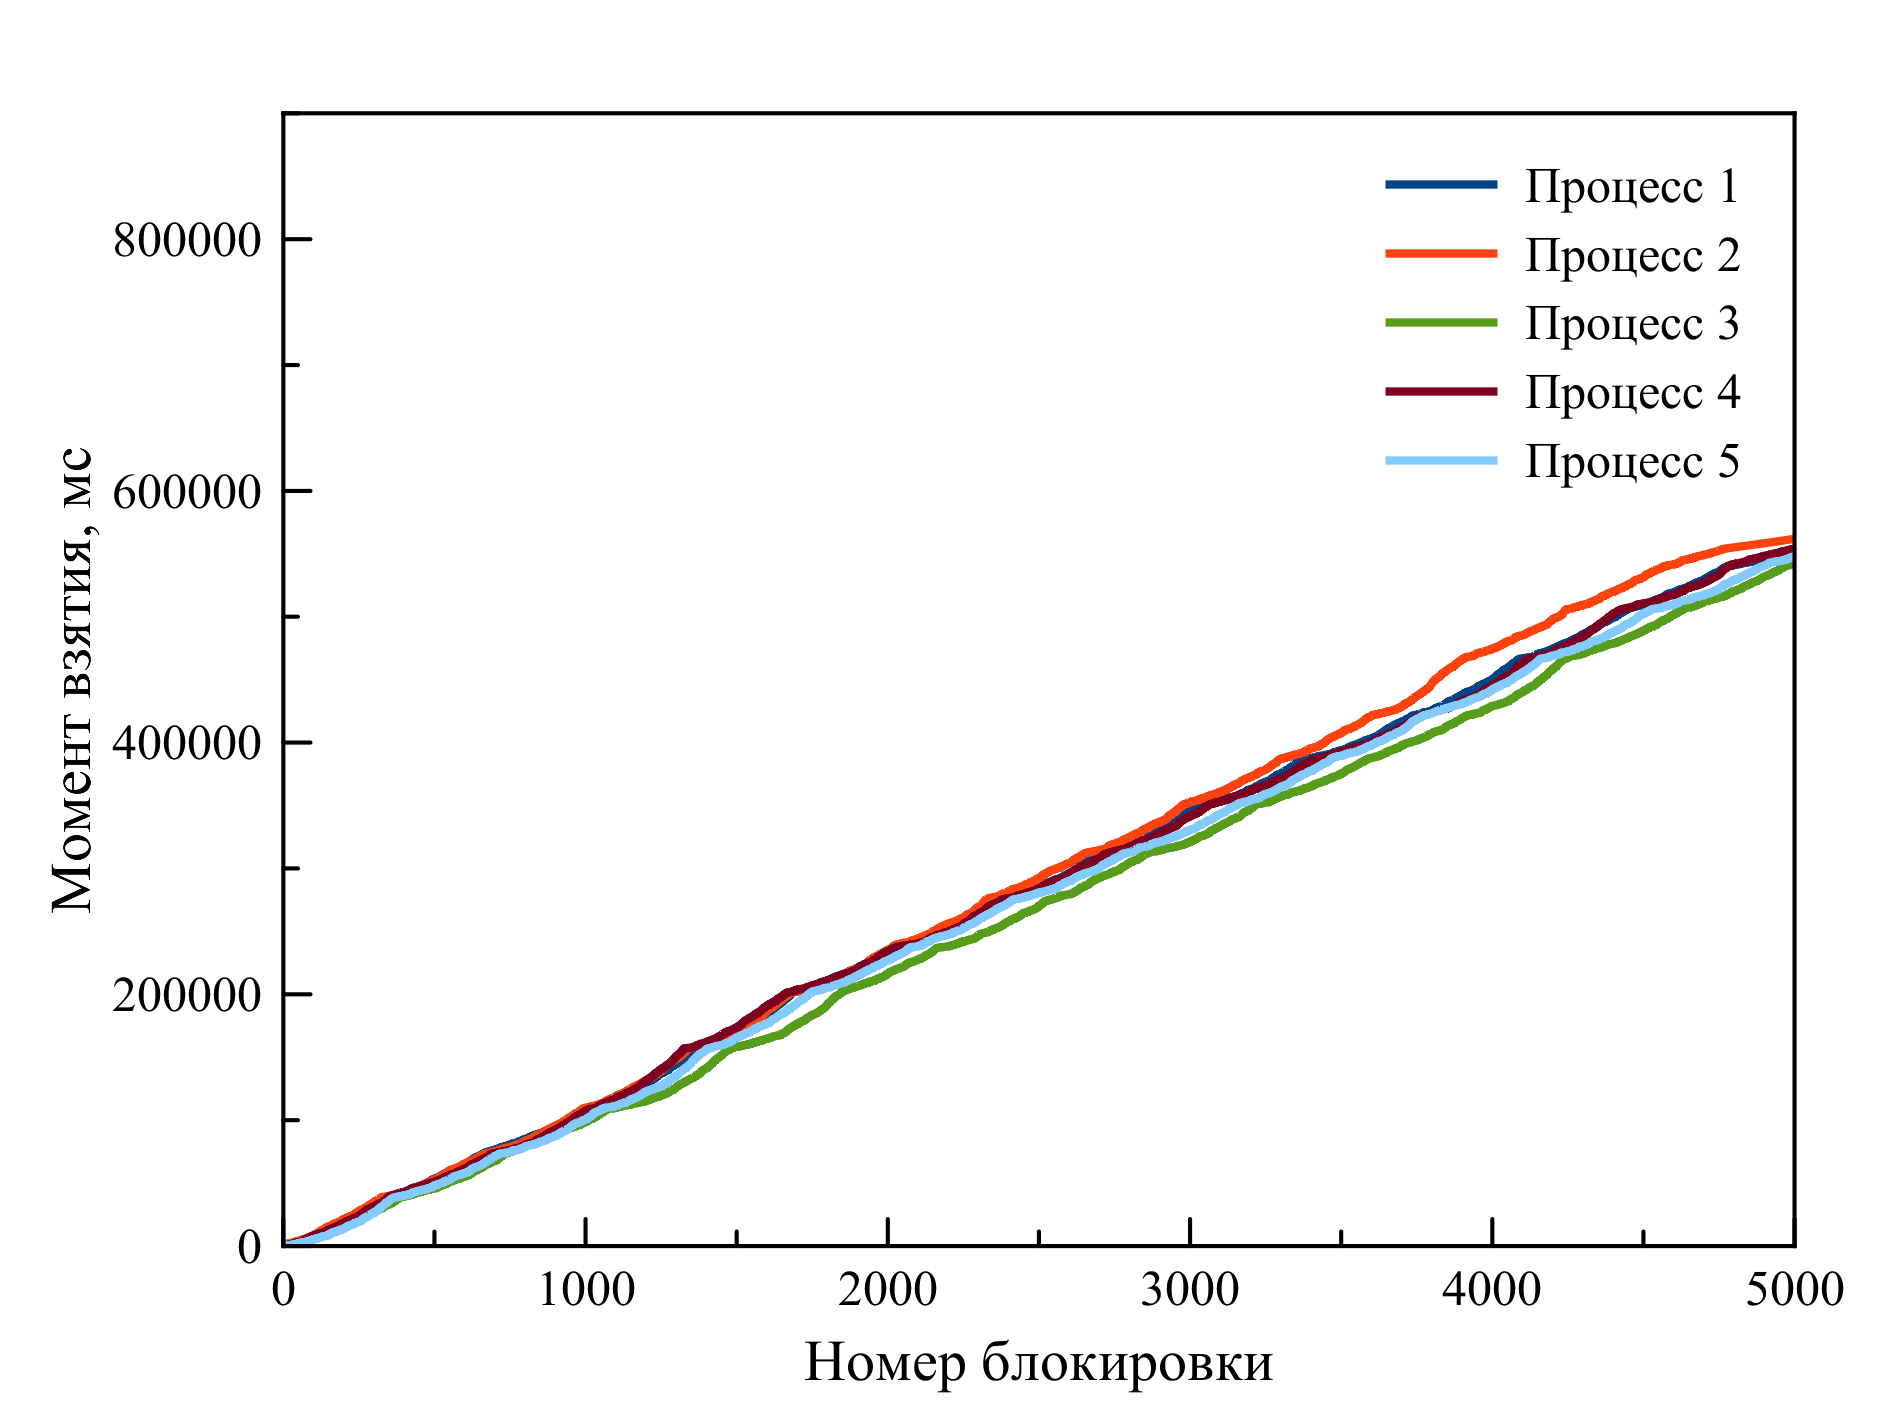
\includegraphics[width=\textwidth]{5_new.png}
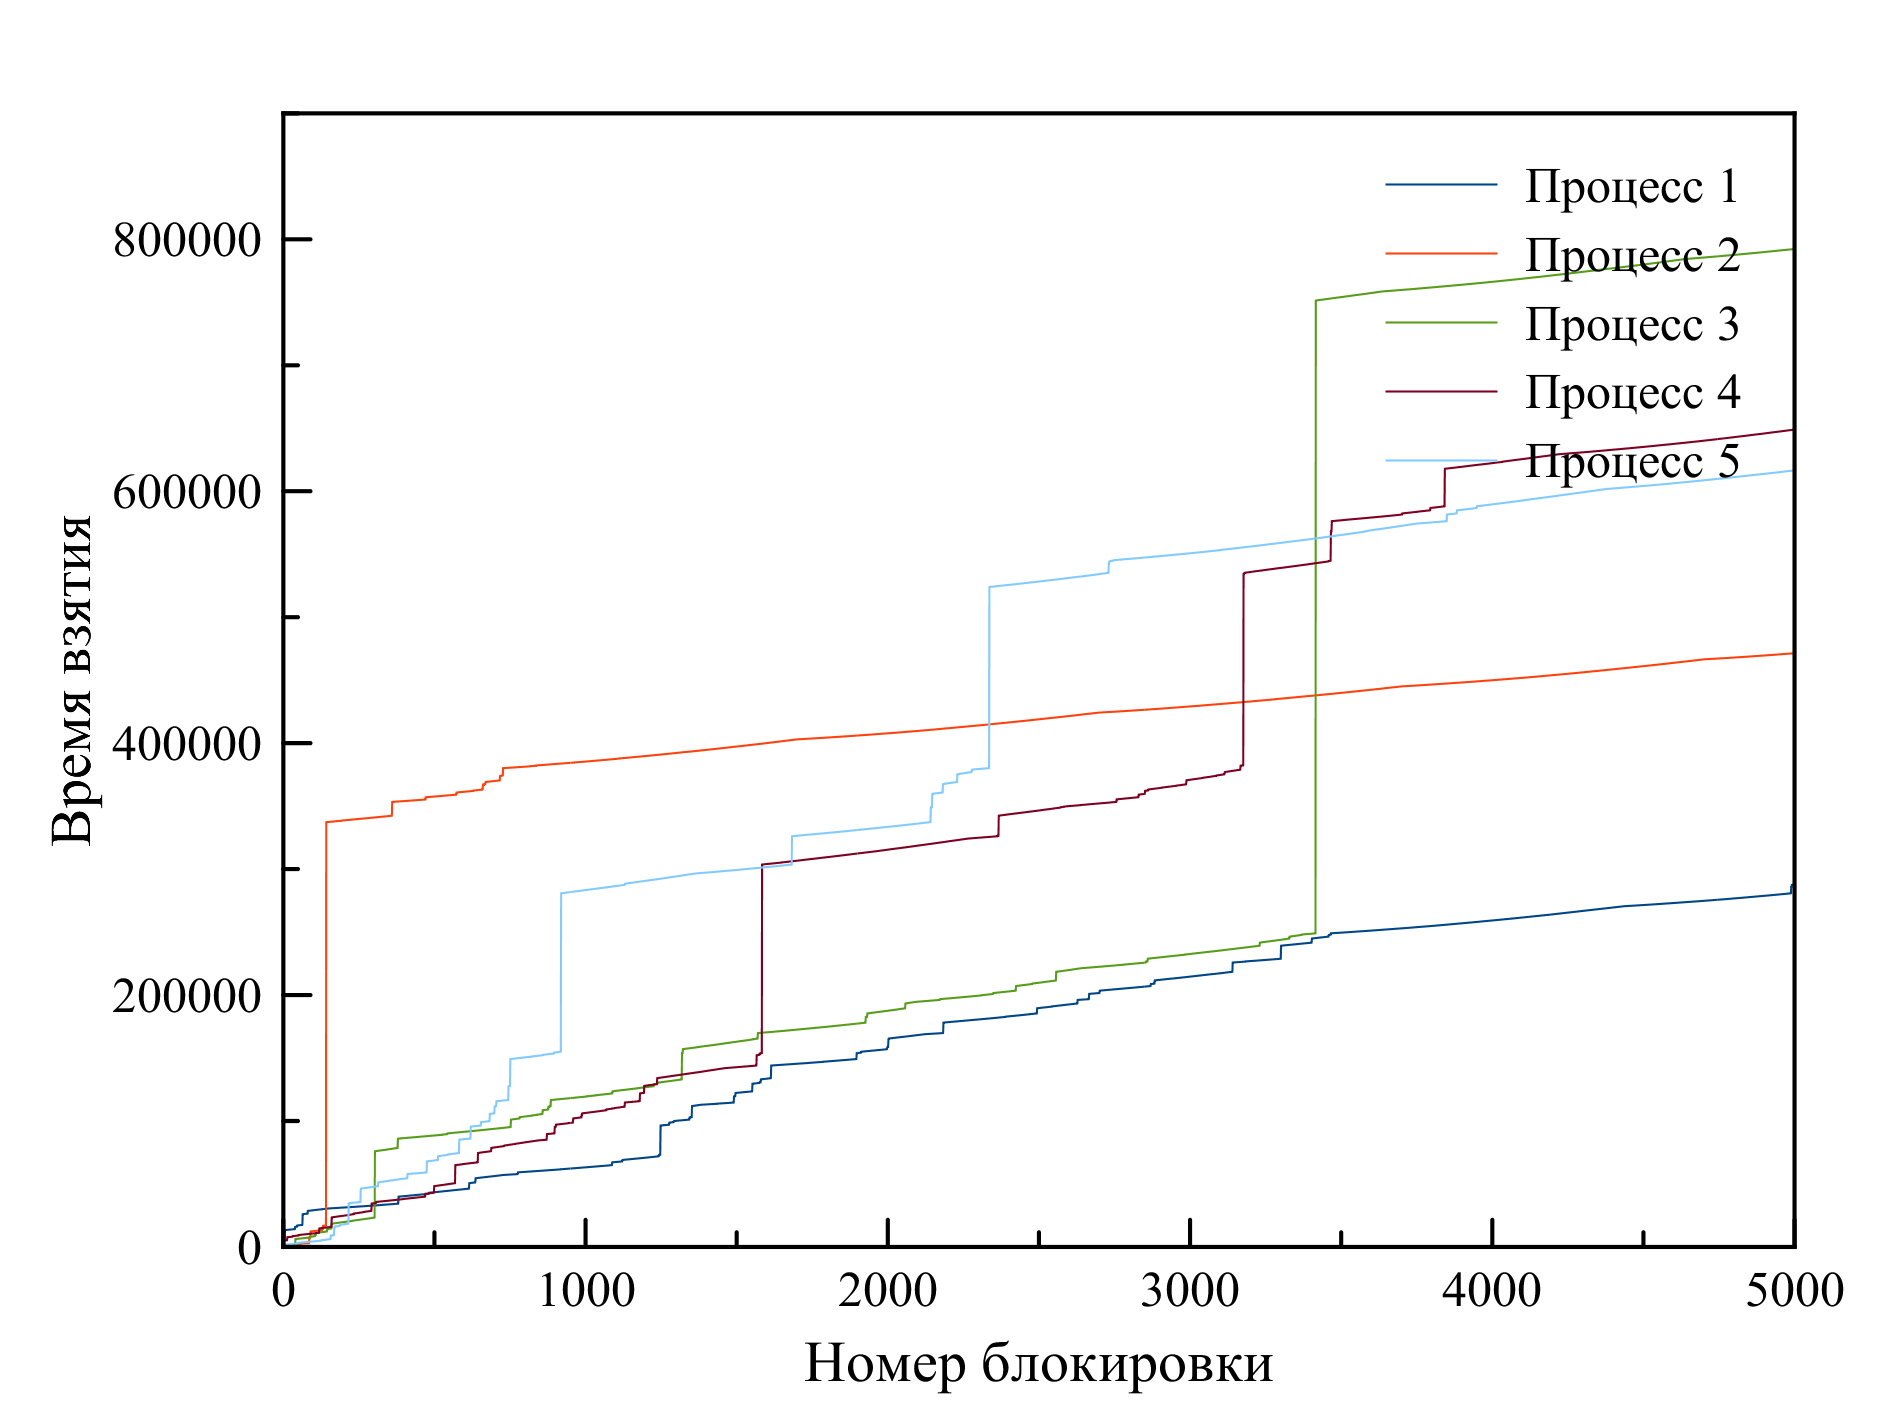
\includegraphics[width=\textwidth]{5_old.png}

Рисунок 1 показывает, что новый алгоритм позволяет потокам брать блокировки равномерно, не отдавая последовательно множество блокировок одному потоку, тем самым максимальное время взятия блокировки минимизируется. Рисунок 2 объясняет, почему старый алгоритм дает такие большие значения максимального времени взятия блокировки: фактически у каждого потока есть несколько больших промежутков времени, в течение которых он непрерывно захватывает множество блокировок, не отдавая ее другим потокам.

